\section{Experiments}
This section describes a series of experiments over a set of benchmarks to determine (1) the effectiveness of the algorithm is quickly witnessing properties of the input program, and (2) how well the algorithm controls the size of the match pair set as the bound $k$ increases.

The benchmark programs come from different sources. Three are derived from actual MPI programs and are used in other works for benchmarking \cite{benchmark:fevs,mpptest_benchmark,DBLP:conf/ppopp/XueLWGCZZV09}.

\begin{compactitem}
\item \textit{Diffu2DNoBa} is modified from the program \textit{Diffusion 2D}, which uses barriers to “partition” the message communication into several sections \cite{benchmark:fevs}. \textit{Diffu2DNoBa} removes the barriers from the original program so deadlocks are present in the new program. The program is also interesting because the messages to any receiver are distributed from a large set of senders.

\item \textit{Pktuse} is executed with only 5 processes -- each of which has a long sequence of messages to be sent to the other processes \cite{mpptest_benchmark}. The program uses wildcard receives only, therefore has a high degree of message non-determinism. 

\item \textit{Floyd} implements the shortest path algorithm for all the pairs of nodes \cite{DBLP:conf/ppopp/XueLWGCZZV09}. Each node communicates only with the immediate following neighbor. The program also has a large set of senders for each receiver. 
\end{compactitem}

The remaining four are synthetic programs created for this study.

\begin{compactitem}
\item \textit{DeepComm} is a simple program with one receiver and 4 senders. The program is designed to have a long sequence of sends for each sender.
This scenario issues only wildcard receives, so that the messages from different senders may race.

\item \textit{MultiM} is an extension to a program in the MCAPI library distribution \cite{DBLP:conf/kbse/HuangMM13}. The program adds extra iterations to the original program to generate longer execution trace. The program uses only wildcard receives and there is an interesting violation of assertion that only occurs in some possible executions.

\item \textit{Mismatch} is designed to contain a communication deadlock in execution. The program interleaves wildcard receives and deterministic receives in the program text. A deterministic receive may be orphaned in program execution leading to a deadlock as all the potential sends it need are matched with the preceding wildcard receives. 

\item \textit{MismatchEx} is an extension to the program in \figref{fig:example} that contains more sends and receives. Similar to the program in \figref{fig:example}, a deadlock may occur in deep execution. 
%No assertions are present in the program.
\end{compactitem}


These programs are tested for three types of properties: assertion violation, zero buffer compatibility and deadlock. 
The deadlock checking relies on a static pattern matcher to identify potential deadlock scenarios \cite{}. 
The experiments here use single pattern match, and the SMT encoding is to witness the feasibility of that match. The same pattern match is used for all experiments on any given deadlock example. 
The initial trace for any input program is generated by MPICH \cite{mpich}, a public implementation of the MPI standard.
The SMT encoding for each test is generated by the existing rules \cite{DBLP:conf/kbse/HuangMM13,HuangNFM15} and is solved by Z3 \cite{demoura:tacas08}. 
The experiments are run on a AMD A8 Quad Core processor with 6 GB of memory running Ubuntu 14.04 LTS. 
%A time limit of 2 hours is set for each test. The test aborts the verification process if it does not complete within the time limit.

\subsection{Effectiveness}

The \textit{effectiveness of property witnessing} are shown in \tableref{table:benchmarks} that divides the tests into three groups, where each group is the tests for a single type of property. Each group is labeled in the first column: ``AssertionV" means assertion violation; ``ZeroCom" means zero buffer compatibility; and ``DL" means deadlock. For each benchmark, $k$ is the minimum value at which the property is witnessed (if the property exists), or the value at which the over-approximated match set is generated (if the property does not exist). 
The column ``\#M" is the number of the generated match pairs for $k$. 
The column ``$\mathrm{Time}_k^\ast$" is the cumulative sum: $\sum_{i=1}^k\mathrm{Time}_i$, where $\mathrm{Time}_i$ is the runtime of checking satisfiability with the generated match pairs for $k=i$.
%The notation ``TO" means ``time out" (exceeding the time limit set for each test). 
The column ``Speed" reports the relative speedup over the running time of simply using the regular over-approximated match pair set: $\mathrm{Time}(Over-approximated) / \mathrm{Time}_k^\ast$.
%The symbol ``--" means that the $\mathrm{Speed}$ can not be computed because the test times out.

\begin{comment}

\begin{savenotes}
\begin{table*}[t]
\begin{center}
\scriptsize
\caption{Tests on Selected Benchmarks}\label{table:benchmarks}
     \begin{threeparttable}
     \def\arraystretch{1.5}
\begin{tabular}{c|c|c|c|p{0.25cm}|c|c|c|p{0.25cm}|c|c|c|c|c|c|c|}
		\cline{2-16}	  
& \multicolumn{3}{c|}{Test Programs} & \multicolumn{4}{c|}{Test 1} & \multicolumn{4}{c|}{Test 2} & \multicolumn{4}{c|}{Test 3}  \\ \cline{2-16}   
        & $Name$ & \#P & \#OP & $k$\tnote{w} & \#M & Time & Speed& $k$ & \#M & Time & Speed & $k$\tnote{+} & \#M & Time & Speed\\ \hline
         \multicolumn{1}{ |c|  }{\multirow{5}{*}{\rotatebox[origin=c]{90}{AssertV}}} 
          &  \textit{Diff2DNoBa} & 16 & 188 & 1\tnote{d} & 514 & 3.508s & 14.86 & 2\tnote{d}& 934 & 31.722s & 1.48 & 3\tnote{d}& 1,066 & 52.131s & 0.59 \\ \cline{2-16}
         \multicolumn{1}{ |c|  }{}&  \textit{DeepComm} & 5 & 180 & 1 & 240 & 0.837s & 1,647 & 5 & 960 & 10.547s & 131 & 15 & 2,760 & 1,379s & 1.00 \\ \cline{2-16}
\multicolumn{1}{ |c|  }{}&  \textit{Pktuse} &5 & 2048 &1 & 1,792 & 180s & $>$40 & 5   &    4,828      & 564s & $>$13 & 128 & 99,328 & TO & -- \\ \cline{2-16}
\multicolumn{1}{ |c|  }{}&  \textit{MultiM} & 3 & 266 & 1 & 500 & 10.892s & 295 & 5 & 1,300 & 24.397s & 132 & 100 & 20,300 & 3,218s & 1.00\\ \cline{2-16}
\multicolumn{1}{ |c|  }{}&  \textit{Floyd} &32 & 528 &1\tnote{d}& 1,928 & 29.925s & 0.97 & 2\tnote{d} &    1,928      & 30.621s & 0.48 & 3\tnote{d} & 1,928 & 29.043s & 0.32 \\ \hline
\hline
        
         \multicolumn{1}{ |c|  }{\multirow{7}{*}{\rotatebox[origin=c]{90}{ZeroCom}}} 
         &  \textit{Diff2DNoBa} & 16 & 188 & 1\tnote{d} & 514 & 1.749s & 3.07 & 2\tnote{d} & 934 & 3.053s & 1.12 & 3\tnote{d}& 1,066 & 5.375s & 0.53 \\ \cline{2-16}
        \multicolumn{1}{ |c|  }{} &  \textit{DeepComm} & 5 & 180 & 1 & 240 & 0.875s & 291 & 5 & 960 & 3.056s & 83 & 15 & 2,760 & 255s & 1.00 \\ \cline{2-16}
\multicolumn{1}{ |c|  }{}&  \textit{Pktuse} &5 & 2048 &1 & 1,792 & 121s & $>$59 & 5   &    4,828      & 449s & $>$16 & 128 & 99,328 & TO & -- \\ \cline{2-16}
\multicolumn{1}{ |c|  }{}&  \textit{MultiM} & 3 & 266 & 1 & 500 & 8.312s & 366 & 5 & 1,300 & 17.843s & 170 & 100 & 20,300 & 3,043s & 1.00\\ \cline{2-16}
\multicolumn{1}{ |c|  }{}&  \textit{Mismatch} &3 & 800 &1 & 204 & 2.904s & 3.06 & 30   &    622      & 3.297s & 2.69 & 50 & 793 & 8.872s & 1.00 \\ \cline{2-16}
\multicolumn{1}{ |c|  }{}&  \textit{MismatchEx} &3 & 296 &1 & 165 & 0.579s & 876  & 20   &    1,687      & 7.433s & 68 & 43 & 3,525 & 507s & 1.00  \\ \cline{2-16}
\multicolumn{1}{ |c|  }{}&  \textit{Floyd} &32 & 528 &1 & 1,928 & 89.032s & 1.02 & 5   &    1,928      & 90.908s & 1.00 & 10 & 1,928 & 91.155s & 1.00 \\ \hline
\hline

         \multicolumn{1}{ |c|  }{\multirow{3}{*}{\rotatebox[origin=c]{90}{DL}}} 
         &  \textit{Diff2DNoBa} & 16 & 188 & 1 & 514 & 3.479s & 13.50 & 2 & 934 & 44.060s & 1.07 & 3 & 1,066 & 46.974s & 1.00 \\ \cline{2-16}
\multicolumn{1}{ |c|  }{}&  \textit{Mismatch} &3 & 800 &1 & 204 & 2.160s & 6.61 & 30   &    622      & 10.061s & 1.42 & 50 & 793 & 14.286s & 1.00 \\ \cline{2-16}
\multicolumn{1}{ |c|  }{}&  \textit{MismatchEx} &3 & 296 &3 & 328 & 1.253s & 27.23 & 20   &    1,687      & 2.438s & 13.99 & 43 & 3,525 & 34.116s & 1.00 \\ \hline

       
\end{tabular}
\begin{tablenotes}
\item[w] $k$ is the minimum value with which the property is witnessed (if the property exists). 
\item[d] The property does not exist for the benchmark.
\item[+] The precise match pairs are over-approximated as $k$ is reached.
\end{tablenotes}
     \end{threeparttable}
\end{center}
\end{table*}
\end{savenotes}

\end{comment}

\begin{savenotes}
\begin{table*}[t]
\begin{center}
\scriptsize
\caption{Tests on Selected Benchmarks}\label{table:benchmarks}
     \begin{threeparttable}
     %\def\arraystretch{1.2}
\begin{tabular}{c|p{1.7cm}|c|c|c|c|c|c|}
		\cline{2-8}	  
& \multicolumn{3}{c|}{Test Programs} & \multicolumn{4}{c|}{Performance}   \\ \cline{2-8}   
        & $Name$ & \#P & \#Calls & $k$ & \#Match & Time & Speed\\ \hline
         \multicolumn{1}{ |c|  }{\multirow{5}{*}{\rotatebox[origin=c]{90}{AssertV}}} 
          &  \textit{Diff2DNoBa}\tnote{d} & 16 & 188 & 3 & 1,066 & 87.361s & 0.59 \\ \cline{2-8}
         \multicolumn{1}{ |c|  }{}&  \textit{DeepComm} & 5 & 180 & 1 & 240 & 0.837s & 1,647 \\ \cline{2-8}
\multicolumn{1}{ |c|  }{}&  \textit{Pktuse} &5 & 2048 &1 & 1,792 & 180s & $>$40 \\ \cline{2-8}
\multicolumn{1}{ |c|  }{}&  \textit{MultiM} & 3 & 266 & 1 & 500 & 10.892s & 295 \\ \cline{2-8}
\multicolumn{1}{ |c|  }{}&  \textit{Floyd}\tnote{d} &32 & 528 & 2 & 1,928 & 60.546s & 0.48 \\ \hline
\hline
        
         \multicolumn{1}{ |c|  }{\multirow{7}{*}{\rotatebox[origin=c]{90}{ZeroCom}}} 
         &  \textit{Diff2DNoBa}\tnote{d}& 16 & 188 & 3& 1,066 & 10.177s & 0.53 \\ \cline{2-8}
        \multicolumn{1}{ |c|  }{} &  \textit{DeepComm} & 5 & 180 & 1 & 240 & 0.875s & 291 \\ \cline{2-8}
\multicolumn{1}{ |c|  }{}&  \textit{Pktuse} &5 & 2048 &1 & 1,792 & 121s & $>$59 \\ \cline{2-8}
\multicolumn{1}{ |c|  }{}&  \textit{MultiM} & 3 & 266 & 1 & 500 & 8.312s & 366 \\ \cline{2-8}
\multicolumn{1}{ |c|  }{}&  \textit{Mismatch} &3 & 800 &1 & 204 & 2.904s & 3.06 \\ \cline{2-8}
\multicolumn{1}{ |c|  }{}&  \textit{MismatchEx} &3 & 296 &1 & 165 & 0.579s & 876  \\ \cline{2-8}
\multicolumn{1}{ |c|  }{}&  \textit{Floyd} &32 & 528 &1 & 1,928 & 89.032s & 1.02 \\ \hline
\hline

         \multicolumn{1}{ |c|  }{\multirow{3}{*}{\rotatebox[origin=c]{90}{DL}}} 
         &  \textit{Diff2DNoBa} & 16 & 188 & 1 & 514 & 3.479s & 13.50 \\ \cline{2-8}
\multicolumn{1}{ |c|  }{}&  \textit{Mismatch} &3 & 800 &1 & 204 & 2.160s & 6.61 \\ \cline{2-8}
\multicolumn{1}{ |c|  }{}&  \textit{MismatchEx} &3 & 296 &3 & 328 & 1.253s & 27.23  \\ \hline 
\end{tabular}
\begin{tablenotes}
\item[d] The property does not exist for the benchmark.
%\item[+] The precise match pairs are over-approximated as $k$ is reached.
\end{tablenotes}
     \end{threeparttable}
\end{center}
\end{table*}
\end{savenotes}



The results show that each property, if existing for the benchmark, is efficiently witnessed by the SMT encoding with the under-approximated match pairs in these benchmarks; it is not known if such early detection takes place in general. The tested properties for all the real programs can be witnessed with $k=1$. 
For example, the assertion violation for the program \textit{Pktuse} can be detected with $k=1$ where the speedup is greater than 40.

For the tests where the properties do not exist in the benchmarks, the results show slow down as expected, but the intent of this work is to improve the ability to find witnesses early rather than to prove correctness. 
For example, three tests are run for the program \textit{Diffu2DNoBa}, where $k$ is incremented from $1$ to $3$. 
The over-approximated match pairs are generated with $k=3$ that can be easily computed based on \thmref{theorem:precise}.


The tests for all the synthetic programs also show the properties can be witnessed with a potential for speed up, even if several tests are required to be run beforehand. For example, the program \textit{MismatchEx} is designed to contain a deadlock deep in an execution. The witness is found after $k$ is incremented to $3$, where the speed up is more than $27$ compared to the runtime with the over-approximated match set for $k=42$. The capability of witnessing properties with a low k-bound is especially helpful for the large programs to be feasible.

 
%also show that the runtime cost of the encoding is highly reduced with the match pairs generated with smaller $k$. For example, the assertion violation test for the program \textit{Diffu2DNoBa} takes 3 seconds to complete for $k=1$, while it takes to 67 seconds to solve the same encoding for $k=5$ only the match set is larger.

%To check zero buffer incompatibility, the precise match pairs are required because a zero buffer incompatible program indicates that all possible schedules are infeasible under zero buffer semantics. 
%As such, the zero buffer incompatibility for the program \textit{Diff2DNoBa} is only detected with $k=\infty$. 
%On the other hand, if any schedule for a program is able to run under zero buffer semantics, the program may never be zero buffer incompatible. As such, if a test shows that a zero buffer encoding is satisfiable for the program, then the program is proved to be zero buffer compatible. 
%The results show that the benchmarks excluding the program \textit{Diff2DNoBa} are zero buffer compatible by testing them with only a small set of match pairs.

%For deadlock detection, a prior static analysis is launched as preprocessing to find all the potential deadlocks in a program. If no potential deadlocks are found, then the SMT encoding is not required. For example, the deadlock test for the program \textit{MuitiM} is unavailable because no potential deadlock is detected.



\subsection{Scalability}
To evaluate how the input $k$ impacts the generated match pairs, the presentation discusses two benchmarks for how the sends are distributed from senders. The benchmarks are outside the set of programs discussed earlier and are defined based on the template program in \figref{fig:Texample}. The template program is simplified to contain only a receiver $p_r$ that issues a sequence of receives, and several senders $p_1,\ldots,p_m$ where each sender issues $N_s$ sends. Therefore, the number of receives in $p_r$ is $N_s\times m$.

\examplefigtemplate

\begin{figure}[!h]
%\begin{minipage}{.5\textwidth}
\centering
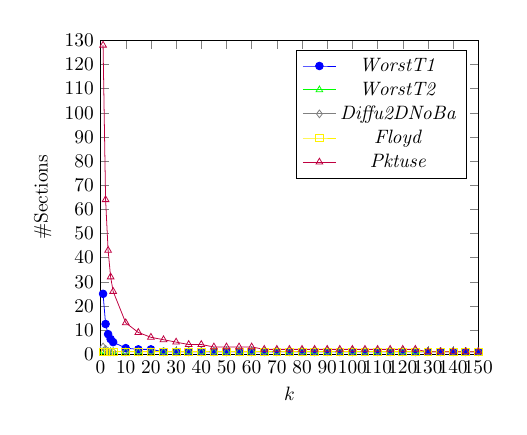
\begin{tikzpicture}[scale=0.7]
\begin{axis}[
    xlabel={$k$},
    ylabel={\#Sections},
    xmin=0, xmax=150,
    ymin=0, ymax=130,
    xtick={0,10,20,30,40,50,60,70,80,90,100,110,120,130,140,150},
    ytick={0,10,20,30,40,50,60,70,80,90,100,110,120,130},
    legend pos= north east,
    %ymajorgrids=true,
    grid style=dashed,
]
 
\addplot[
    color=blue,
    mark=*,
    ]
    coordinates {
    (1,25)(2,12.5)(3,8.3)(4,6.25)(5,5)(10,2.5)(15,2)(20,2)(25,1)(30,1)(35,1)(40,1)(45,1)(50,1)(55,1)(60,1)(65,1)(70,1)(75,1)(80,1)(85,1)(90,1)(95,1)(100,1)(105,1)(110,1)(115,1)(120,1)(125,1)(130,1)(135,1)(140,1)(145,1)(150,1)
    };

%\addplot[
  %  color=red,
   % mark=square,
   % ]
   % coordinates {
    %(1,25)(2,12.5)(3,8.3)(4,6.25)(5,5)(10,2.5)(15,2)(20,2)(25,1)(30,1)(35,1)(40,1)(45,1)(50,1)(55,1)(60,1)(65,1)(70,1)(75,1)(80,1)(85,1)(90,1)(95,1)(100,1)(105,1)(110,1)(115,1)(120,1)(125,1)(130,1)(135,1)(140,1)(145,1)(150,1)
   % };

\addplot[
    color=green,
    mark=triangle,
    ]
    coordinates {
    (1,1)(2,1)(3,1)(4,1)(5,1)(10,1)(15,1)(20,1)(25,1)(30,1)(35,1)(40,1)(45,1)(50,1)(55,1)(60,1)(65,1)(70,1)(75,1)(80,1)(85,1)(90,1)(95,1)(100,1)(105,1)(110,1)(115,1)(120,1)(125,1)(130,1)(135,1)(140,1)(145,1)(150,1)
    };
    
\addplot[
    color=gray,
    mark=diamond,
    ]
    coordinates {
    (1,3)(2,2)(3,1)(4,1)(5,1)(10,1)(15,1)(20,1)(25,1)(30,1)(35,1)(40,1)(45,1)(50,1)(55,1)(60,1)(65,1)(70,1)(75,1)(80,1)(85,1)(90,1)(95,1)(100,1)(105,1)(110,1)(115,1)(120,1)(125,1)(130,1)(135,1)(140,1)(145,1)(150,1)
    };
    
    \addplot[
    color=yellow,
    mark=square,
    ]
    coordinates {
    (1,1)(2,1)(3,1)(4,1)(5,1)(10,1)(15,1)(20,1)(25,1)(30,1)(35,1)(40,1)(45,1)(50,1)(55,1)(60,1)(65,1)(70,1)(75,1)(80,1)(85,1)(90,1)(95,1)(100,1)(105,1)(110,1)(115,1)(120,1)(125,1)(130,1)(135,1)(140,1)(145,1)(150,1)
    };
    
      \addplot[
    color=purple,
    mark=triangle,
    ]
    coordinates {
    (1,128)(2,64)(3,43)(4,32)(5,26)(10,13)(15,9)(20,7)(25,6)(30,5)(35,4)(40,4)(45,3)(50,3)(55,3)(60,3)(65,2)(70,2)(75,2)(80,2)(85,2)(90,2)(95,2)(100,2)(105,2)(110,2)(115,2)(120,2)(125,2)(130,1)(135,1)(140,1)(145,1)(150,1)
    };    
    
    \legend{\textit{WorstT1},\textit{WorstT2},\textit{Diffu2DNoBa},\textit{Floyd},\textit{Pktuse}}
 
\end{axis}
 
\end{tikzpicture}
%\end{minipage}

\caption{The number of divided sections of varying the input $k$.}
\label{fig:relation:section}
\end{figure}

\begin{figure}[!h]
\centering
%\begin{minipage}{.55\textwidth}
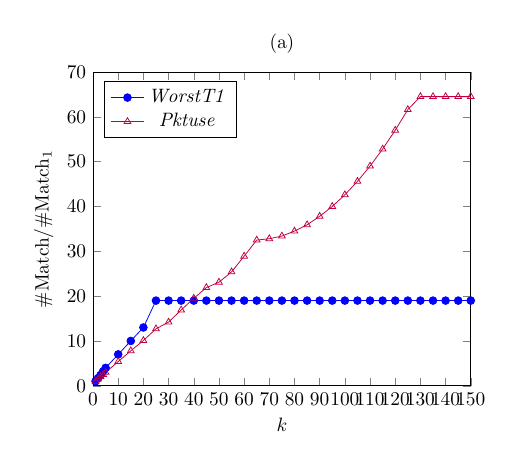
\begin{tikzpicture}[scale=0.7]
\begin{axis}[
   title = {(a)},
    xlabel={$k$},
    ylabel={\#Match$/$\#$\mathrm{Match}_1$},
    xmin=0, xmax=150,
    ymin=0, ymax=70,
    xtick={0,5,10,15},
    xtick={0,10,20,30,40,50,60,70,80,90,100,110,120,130,140,150},
    ytick={0,10,20,30,40,50,60,70},
    legend pos=  north west,
    %ymajorgrids=true,
    grid style=dashed,
]   

    
\addplot[
    color=blue,
    mark=*,
    ]
    coordinates {
    (1,1)(2,1.7)(3,2.4)(4,3.2)(5,4)(10,7)(15,10)(20,13)(25,19)(30,19)(35,19)(40,19)(45,19)(50,19)(55,19)(60,19)(65,19)(70,19)(75,19)(80,19)(85,19)(90,19)(95,19)(100,19)(105,19)(110,19)(115,19)(120,19)(125,19)(130,19)(135,19)(140,19)(145,19)(150,19)
    };
    

    
    \addplot[
    color=purple,
    mark=triangle,
    ]
    coordinates {
    (1,1)(2,1.5)(3,2)(4,2.5)(5,2.98)(10,5.4)(15,7.8)(20,10.1)(25,12.7)(30,14.2)(35,16.9)(40,19.5)(45,21.9)(50,23.1)(55,25.4)(60,28.9)(65,32.5)(70,32.8)(75,33.4)(80,34.5)(85,35.9)(90,37.8)(95,40)(100,42.6)(105,45.6)(110,49)(115,52.8)(120,57)(125,61.6)(130,64.5)(135,64.5)(140,64.5)(145,64.5)(150,64.5)
    };
    
    \legend{\textit{WorstT1},\textit{Pktuse}}
\end{axis}
\end{tikzpicture}
%\end{minipage}

%\begin{minipage}{.55\textwidth}
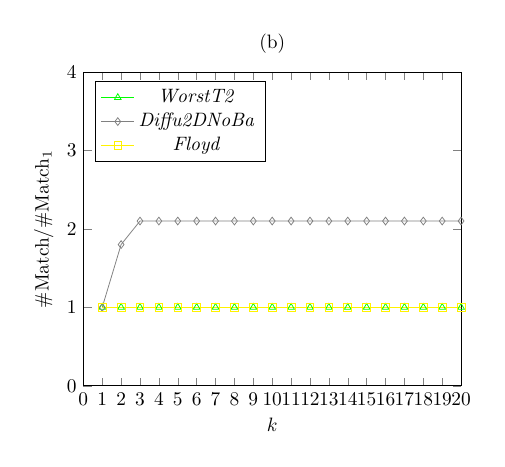
\begin{tikzpicture}[scale=0.7]
\begin{axis}[
   title = {(b)},
    xlabel={$k$},
    ylabel={\#Match$/$\#$\mathrm{Match}_1$},
    xmin=0, xmax=20,
    ymin=0, ymax=4,
    xtick={0,5,10,15},
    xtick={0,1,2,3,4,5,6,7,8,9,10,11,12,13,14,15,16,17,18,19,20},
    ytick={0,1,2,3,4},
    legend pos=  north west,
    %ymajorgrids=true,
    grid style=dashed,
]   
    
     %\addplot[
    %color=red,
   % mark=square,
    %]
    %coordinates {
%(1,1)(2,1)(3,1)(4,1)(5,1)(10,1)(15,1)(20,1)(25,1)(30,1)(35,1)(40,1)(45,1)(50,1)(55,1)(60,1)(65,1)(70,1)(75,1)(80,1)(85,1)(90,1)(95,1)(100,1)(105,1)(110,1)(115,1)(120,1)(125,1)(130,1)(135,1)(140,1)(145,1)(150,1)
 %   };
    
    \addplot[
    color=green,
    mark=triangle,
    ]
    coordinates {
    (1,1)(2,1)(3,1)(4,1)(5,1)(6,1)(7,1)(8,1)(9,1)(10,1)(11,1)(12,1)(13,1)(14,1)(15,1)(16,1)(17,1)(18,1)(19,1)(20,1)(25,1)(30,1)(35,1)(40,1)(45,1)(50,1)(55,1)(60,1)(65,1)(70,1)(75,1)(80,1)(85,1)(90,1)(95,1)(100,1)(105,1)(110,1)(115,1)(120,1)(125,1)(130,1)(135,1)(140,1)(145,1)(150,1)
    };
    
    \addplot[
    color=gray,
    mark=diamond,
    ]
    coordinates {
    (1,1)(2,1.8)(3,2.1)(4,2.1)(5,2.1)(6,2.1)(7,2.1)(8,2.1)(9,2.1)(10,2.1)(11,2.1)(12,2.1)(13,2.1)(14,2.1)(15,2.1)(16,2.1)(17,2.1)(18,2.1)(19,2.1)(20,2.1)(25,2.1)(30,2.1)(35,2.1)(40,2.1)(45,2.1)(50,2.1)(55,2.1)(60,2.1)(65,2.1)(70,2.1)(75,2.1)(80,2.1)(85,2.1)(90,2.1)(95,2.1)(100,2.1)(105,2.1)(110,2.1)(115,2.1)(120,2.1)(125,2.1)(130,2.1)(135,2.1)(140,2.1)(145,2.1)(150,2.1)
    };
    
    \addplot[
    color=yellow,
    mark=square,
    ]
    coordinates {
    (1,1)(2,1)(3,1)(4,1)(5,1)(6,1)(7,1)(8,1)(9,1)(10,1)(11,1)(12,1)(13,1)(14,1)(15,1)(16,1)(17,1)(18,1)(19,1)(20,1)(25,1)(30,1)(35,1)(40,1)(45,1)(50,1)(55,1)(60,1)(65,1)(70,1)(75,1)(80,1)(85,1)(90,1)(95,1)(100,1)(105,1)(110,1)(115,1)(120,1)(125,1)(130,1)(135,1)(140,1)(145,1)(150,1)
    };
    
    \legend{\textit{WorstT2},\textit{Diffu2DNoBa},\textit{Floyd}}
\end{axis}
\end{tikzpicture}
%\end{minipage}

\caption{The relative growth of the number of match pairs of varying the input $k$, where $\mathrm{Match}_1$ is the number of the generated match pairs for $k=1$.}
\label{fig:relation:match}
\end{figure}

The first benchmark, \textit{WorstT1}, is constructed by restricting all the receives in \figref{fig:Texample} to be wildcard, which implies the worst case of message non-determinism. Also, let $m=4$ and $N_s = 25$ for the program so there are more than one sections divided for a set of possible $k$-bound. In contrast, the best case of message non-determinism is a program that only contains deterministic receives. As such, the matches for the best case are deterministic.
%In contrast, the second benchmark \textit{BestT1} is the best case of message non-determinism, where the program text is similar to \textit{WorstT1} only the receives are deterministic. 

The second benchmark, \textit{WorstT2}, is related to the worst case of wide communication. Wide communication in this context means that the sender only sends one message to the receiver. The program is constructed by setting $N_s=1$ and $m=100$. As for the best case of wide communication, the program has to contain only the deep communication where a receiver has exactly one sender. The presentation does not discuss this case as the matches are deterministic such that the messages are received in a fixed FIFO order. 

Given the two worst-case programs, the presentation discusses how the number of sections and the number of match pairs grow as $k$ increases for the two cases. 
The relationship between the number of sections and $k$ is illustrated in \figref{fig:relation:section}, and the relationship between the number of match pairs and $k$ is illustrated in \figref{fig:relation:match}.
Note that the values of y-axis in \figref{fig:relation:match} are computed by dividing the number of match pairs for any $k$ by the number of match pairs for $k=1$.

\figref{fig:relation:section} shows that the growth of the number of sections is not linear for the program \textit{WorstT1}. As such, incrementing $k$ may not be meaningful if the number of sections does not change. The algorithm only outputs the generated match pairs to the SMT encoding if the number of sections has changed.
Since the number of the generated match pairs per section is also non-linear according to the complexity of $\mathrm{MatchApprox}$ in \algoref{algo:main}, the total number of the match pairs for \textit{WorstT1} in \figref{fig:relation:match} (a) has a sharp growth between small values of $k$, and then grows more gently until it reaches the limit, which represents the over-approximated match pairs. This observation demonstrates that the algorithm scales for a small range of $k$ where the generated match set is small.

%The program \textit{BestT1} has the same growth of the number of sections with that for \textit{WorstT1} (not shown in \figref{fig:relation} (a)) because the send distribution has no difference between the two programs. 
%Since all the receives are deterministic in the program \textit{BestT1} indicating the matches are also deterministic, the number of the match pairs in \figref{fig:relation} (b) does not grow across $k$.

For the program \textit{WorstT2}, \figref{fig:relation:section} shows that the number of sections is always one as expected because only one section can be divided for wide communication. 
As such, the total number of match pairs for \textit{WorstT2} in \figref{fig:relation:match} (b) does not change. 

Based on the discussion of message non-determinism and wide communication, the synthetic programs discussed earlier can be grouped. The programs \textit{DeepComm} and \textit{MultiM} are close to the worst case of message non-determinism as only wildcard receives are employed in both programs. For the wide communication, no synthetic program is close to the worst case. Instead, all the programs show a certain degree of deep communication. 

The real programs can also be classified for message non-determinism and wide communication. \figref{fig:relation:section} and \figref{fig:relation:match} further plot the relations for the real programs. 
The programs \textit{Diff2DNoBa} and \textit{Floyd} uses more wide communication, therefore, their growths in \figref{fig:relation:match} rapidly reach the bound of match pairs. In contrast, the program \textit{Pktuse} employs a large degree of deep communication with many wildcard receives. As such, \textit{Pktuse} in \figref{fig:relation:match} (a) gradually grows to the bound as $k$ increases to $128$.
Thefore, the presentation demonstrates that the algorithm is able to scale to a program with a high degree of message non-determinism and a high degree of deep communication.


